\documentclass[5p,sort&compress]{elsarticle}		
% 5p gir 2 kolonner pr side. 1p gir 1 kolonne pr side.
% Valget sort&compress gjør at referansen [1,2,3] settes som [1-3]. 
% Andre innstillinger for "klassen" elsarticle finnes i dokumentasjonen på CTAN (http://www.ctan.org/pkg/elsarticle)

% Klassen elsarticle er laget for bruk i engelskspråklige tiksskrift. I blokken under bruker vi litt lavnivå TeX-magi for å redefinere bunnteksten på tittelsiden. Ikke bekymre deg for denne biten med kode, det som kommer lengere nede i dokumentet er lettere å forstå!
\makeatletter
\def\ps@pprintTitle{%
 \let\@oddhead\@empty
 \let\@evenhead\@empty
 \let\@evenfoot\@oddfoot}
\makeatother

% Encoding for input i tex-filen og encoding for output i pdf-filen
\usepackage[utf8]{inputenc}
\usepackage[T1]{fontenc}
\usepackage{textcomp}
\usepackage{amsmath}
\usepackage{float}

\numberwithin{equation}{subsection}


% Last inn en font-pakke. Her bruker vi standard-fonten til LaTeX. 
\usepackage{lmodern}

% LaTeX gjør mye av typografien for deg, blant annet orddeling ved linjeskift og automatisk utfylling av endel tekst. For å kunne gjøre dette må kompilatoren vite hvilket språk dokumentet er skrevet på. 
\usepackage[fixlanguage]{babelbib}
% Til tross for at vi har fortalt kompilatoren at vi skriver på norsk må vi fortelle den eksplisitt at vi ønsker at seksjonen "abstract" skal kalles "sammendrag"
\renewenvironment{abstract}{\global\setbox\absbox=\vbox\bgroup
\hsize=\textwidth\def\baselinestretch{1}%
\noindent\unskip\textbf{Abstract}
\par\medskip\noindent\unskip\ignorespaces}
{\egroup}

% Mikrotypografiske optimeringer
\usepackage[babel=true]{microtype}

% AMS-utvidelsene for å håndtere matematikk
\usepackage{amsmath}
\usepackage{amssymb}
\usepackage{bm}

% Måltall og enheter er spesielle typografiske dyr som reguleres av strenge regler. For å gjøre det enklere å håndtere tall og enheter på riktig måte bruker vi pakken siunitx.
\usepackage{siunitx}
% Vi tilpasser standardinstillingene til pakken til norske regler. 


% Figurer og tabeller
\usepackage{graphicx} % Denne pakken er standard for å kunne laste inn figurfiler med ulike formater
% Løsne opp på de alt for strenge standardinstillingene for plassering av figurer og tabeller (floats) i LaTeX-kjernen
\renewcommand{\topfraction}{.85}
\renewcommand{\bottomfraction}{.7}
\renewcommand{\textfraction}{.15}
\renewcommand{\floatpagefraction}{.66}
\setcounter{topnumber}{3}
\setcounter{bottomnumber}{2}
\setcounter{totalnumber}{10}
\usepackage{flafter} % For å plassere floats i PDFen første sted LaTeX tillater etter det punktet de er definert i TeX-filen. Om du definerer figuren i TeX-filen rett etter at du refererer til den for første gang vil denne pakken sørge for at de fleste floats havner på greie steder
\usepackage{booktabs} % Denne pakken gir tilgang på endel ekstra kommandoer som legger til rette for god skikk og bruk i tabellformatering.
\usepackage{multirow}
\usepackage[font=small,labelfont=bf]{caption}	% Justering av LaTeX standarder for figurtekst og tabelltekst.

% Hyperreferanser
\usepackage[colorlinks=true,allcolors=blue]{hyperref}
% Noen av navnene for autoreferanser mangler på norsk, så vi ordner opp i det.

% Vi endrer fonten som brukes for URLer til den vanlige tekstfonten.
\urlstyle{same}

%%%%%%%%%%%%%%%%%%%%%%%%%%%%%%%%%%%%%
% Selve dokumentet
%%%%%%%%%%%%%%%%%%%%%%%%%%%%%%%%%%%%%

\begin{document}

% I "front matter" angir vi formalia knyttet til dokumentet -- tittel, forfatter, tilknytning og sammendrag
\begin{frontmatter}

\title{Diffusion, Waves, Shock and Mathematical Subtleties ...}

% I forfatterlisten legger vi inn "ikke-brytende" mellomrom etter initialene
\author{Emil~S.~Spasov}

\address{Department of Physics, Norwegian University of Science and Technology, 7491 Trondheim.}

\begin{abstract}

This report investigates the numerical solutions to fundamental physics equations - the Diffusion, Wave, and Advection equations. We study the nonlinear behaviour of Hopf’s equation and the formation of shock. Utilizing finite difference methods, we analyze these systems under various initial and boundary conditions and explore numerical stability, precision, and accuracy of the solutions, while taking in consideration the trade-offs between computational efficiency and the quality of numerical results. Comparative analysis with analytical solutions underscores the effectiveness of the numerical approaches. Future research should focus on refining these numerical techniques, as well as exploring new ones, to enhance their applicability to complex physical systems.

\end{abstract}

\end{frontmatter}


\section{Introduction}
Partial differential equations (PDEs) are fundamental in modeling various physical, biological, and social phenomena. Analytical solutions of PDEs are often difficult or even impossible to find due to the complexity of the equations, especially for domains with specific geometries or boundary conditions.

This issue makes us resort to numerical methods for an approximate solution. These methods, however, often come with significant issues in terms of precision, accuracy and stability. A compromise between computational efficiency and accuracy is required due to the physical restraints imposed by the hardware.

The focus in this report will be on three of the most common physics equations, namely the Diffusion, Wave and Advection equations as well as the nonlinear Hopf's equation (also known as the Inviscid Burgers' equation).

Different ways to model them numerically using finite difference methods in order to find approximate solutions and study the quality of the results are used. We study the 'shock' in the case of Hopf's equation. In this context, a shock refers to a situation where the solution develops a discontinuity in the field variable, typically the velocity field, despite the initial condition being smooth. 

\section{Theory}
Most of the PDEs we encounter in everyday life do not have analytical solutions for the general case, but it is possible to derive such for specific conditions where the problem simplifies sufficiently. Even though this report focuses on computational methods, analytical solutions can help us verify and optimize our models. We will view each of the 4 equations separately and analyze them. 

\subsection{Diffusion equation}
The diffusion equation is used to describe different phenomena, like the evolution of the density of a substance in a solvent or temperature in a medium. Let us assume for simplicity that $u(x,t)$  is the density of some 'mass' at position $x$ and at time $t$. We consider a 1D problem.
The conservation of 'mass' is given by the equation
\begin{equation}
    \frac{\partial u}{\partial t} + \nabla \cdot \mathbf{J} = 0 \text{ and }    \mathbf{J} = -D \nabla u 
    \label{conservation_eq}
\end{equation}
where J is the flux vector field as described by Fick's law. Combining the two equations and simplifying to 1D we obtain the diffusion equation given by:
\begin{equation}
\frac{\partial u}{\partial t} = \frac{\partial}{\partial x} \left( D \frac{\partial u}{\partial x} \right)
\label{eq:diffusion}
\end{equation}
Where $D$ is the diffusion constant with dimension $ \frac{\text{length}^2}{\text{time}}$, which might in principle depend on the position,
time and even the density $u$ but the latter will lead to non-linear PDE. In this problem we will work only with $D$ - constant and as function of the position $D(x)$. There exist analytical solutions for the diffusion equation for different boundary conditions. We will compare them to the numerical solutions and check the validity of our results.

We consider the initial condition
\begin{equation}
u(x,0) = \Tilde{u}_0 \delta(x-x_0)
\label{eq:diff_IC}
\end{equation}
which models a sudden spill of 'mass' $\Tilde{u}_0$ concentrated in an infinitely small volume at $x = x_0$. $\delta (x-x_0)$ denotes the Dirac delta distribution centered at $x = x_0$ having a unit of inverse the argument, in this case - length$^{-1}$. Hence, for equation (\ref{eq:diffusion}) to be valid $\Tilde{u}_0$ must have a unit of [u]$\cdot$length or in the case of a sudden spill of mass with density $u$, $\Tilde{u}_0$ will have a unit of [mass]. Furthermore, assume that the only source was the one at time $t = 0$, meaning there is no flux going in the system for $t>0$. The rate of change of the total 'mass' with respect of time is given by:
\begin{equation}
    \frac{d}{dt}\int_a^b u(x,t) dx = \left. \left( D\frac{\partial u}{\partial x}\right)\right|_{x=b} -  \left. \left( D\frac{\partial u}{\partial x}\right)\right|_{x=a}
    \label{eq:mass_conservation}
\end{equation}

Let's for now assume constant diffusivity \textbf{D = \text{const}}. To solve the diffusion equation we can use different boundary conditions. Firstly let's discuss the unbounded case which can represent something like a drop of ink in a big pool of water. Then the concentration of ink at the boundary is $lim_{x\rightarrow\infty} u(x,t) = 0$. In the unbounded case there exist an analytical solution \cite{assignment}.
% The diffusion equation in the unbounded case has the following analytical solution:
% \begin{equation}
% u(x,t) = \frac{\Tilde{u}_0}{\sqrt{4\pi D t}} \exp\left( -\frac{(x-x_0)^2}{4 D t}\right)
% \label{eq:analytical_diff_unbounded}
% \end{equation}
Valid for $x \in \mathbb{R}$ and $t > 0$. \cite{assignment}

For a system bounded to an interval $[a,b]$ we can consider two types of boundary conditions in the 1D case:
\begin{itemize}
    \item Dirichlet boundary conditions, specify the value of $u$ on the boundary:
    \begin{equation}
    u(a,t) = u_a(t) \text{, } u(b,t) = u_b(t)
    \label{eq:dirichlet}
    \end{equation}

    \item Neumann boundary conditions, specify the gradient of $u$ normal to the boundary (i.e., the flux):
    \begin{equation}
    \partial_x u(a,t) = v_a(t) \text{, } \partial_x u(b,t) = v_b(t)
    \label{eq:neumann}
    \end{equation}
\end{itemize}

To simulate perfectly absorbent boundaries we can use the Dirichlet condition (\ref{eq:dirichlet}) setting $u_a = u_b = 0$. We see that it agrees with the conservation of 'mass' given by (\ref{eq:mass_conservation}), where the two terms on the right side represent the flux of mass out of the system. Hence we expect the total mass in the system to go towards zero as $t \rightarrow \infty$.

We can also imagine modelling a drop of ink in a glass of water as having reflective boundaries where there is no flux through the walls. For this case we can consider Neumann B.C. (\ref{eq:neumann}) and set $v_a = v_b = 0$. Setting these values in equation (\ref{eq:mass_conservation}) we see that the rate of change of the mass with respect to time is 0, therefore we expect that the mass is always constant $\int u(x,t)dx = \Tilde{u}_0$ for all $t$.

For the reflective and absorbing boundary problems with constant D, a domain $[0, L]^2$, and $t>0$, analytic solutions also exists given in the assignment text \cite{assignment}. 

% \begin{equation}
% u(x,t) = \Tilde{u}_0 \sum_{n=0}^{\infty}\exp\left(-\left( \frac{n\pi}{L}\right)^2 Dt\right) v_n(x_0)v_n(x)
% \label{eq:analytical_diff_bounded}
% \end{equation}
% where the $(v_n)_{n\in \mathbb{N}}$ are the so called, eigenfunctions of the diffusion operator satisfying the boundary conditions \cite{assignment}, and defined as: 
% \begin{itemize}
%     \item Absorbing boundaries
%     \begin{equation}
%         u_n(x) = 
%         \begin{cases} 
%         0 & \text{for } n = 0, \\
%         \sqrt{\frac{2}{L}} \sin\left(\frac{n \pi x}{L}\right) & \text{for } n > 0.
%         \end{cases}
%     \label{eq:absorbing_eigenf}
%     \end{equation}
    
%     \item Reflective boundaries
%     \begin{equation}
%         u_n(x) = 
%         \begin{cases} 
%         \sqrt{\frac{1}{L}} & \text{for } n = 0, \\
%         \sqrt{\frac{2}{L}} \sin\left(\frac{n \pi x}{L}\right) & \text{for } n > 0.
%         \end{cases}
%     \label{eq:reflecting_eigenf}
%     \end{equation}
% \end{itemize}

Let's relax our initial assumption of constant diffusivity defining the $D$ as a step function of the position $x$. The diffusion equation the has the following form:
    \begin{equation}
        D(x) = 
        \begin{cases} 
        D_{+} & \text{for } n \ge 0, \\
        D_{-} & \text{for } n < 0. 
        \end{cases}
    \label{eq:step_diff}
    \end{equation}
where $D_+, D_- \in \mathbb{R_+}$. This could model for example the diffusion of temperature in a bar
composed of one material, say copper, on one half and another one, say iron, on the other half. This problem has an analytical solution for the unbounded case for $x\in\mathbb{R}$ and $t>0$ given by \cite{assignment}.
% \begin{equation}
%     \frac{u(x,t)}{\Tilde{u}_0} =
%         \begin{cases} 
%             \frac{A_+(t)}{\sqrt{4\pi D_+ t}} \exp\left( -\frac{(x-x_0)^2}{4 D_+ t}\right) & \text{for } n \ge 0, \\
%             \frac{A_-(t)}{\sqrt{4\pi D_- t}} \exp\left( -\frac{(x-x_0)^2}{4 D_- t}\right) & \text{for } n < 0. 
%         \end{cases}
% \label{eq:analytical_step_diff}
% \end{equation}
% where $\varepsilon_{\pm} = \text{erf}\left(\frac{x_0}{\sqrt{4 D_\pm t}}\right)$ and
% \small
% \begin{align*}
% A_+(t) = 2\left[1+ \varepsilon_+ + \sqrt{\frac{D_-}{D_+}} \exp\left( \frac{(D_+ - D_-)x_0^2}{4 D_+ D_- t}\right)(1-\varepsilon_-)\right]^{-1}
% \end{align*}

% \begin{align*}
%     A_-(t) = A_+(t) \sqrt{\frac{D_-}{D_+}} \exp\left( \frac{(D_+ - D_-)x_0^2}{4 D_+ D_- t}\right)
% \end{align*}
\normalsize
\subsection{Wave equation}
The wave equation is used to model wave phenomena such a mechanical wave propagating along string, deformation wave on a membrane, pressure waves in a gas and even electromagnetic waves to some extend. It is given by the equation
\begin{equation}
\frac{\partial^2 u}{\partial t^2} -c^2 \nabla u = 0
\label{eq:wave}
\end{equation}
Here $|c|$ is the speed of the wave. For better visualisation we will study a 2D case.

We consider the following initial and boundary conditions:
\begin{align}
    u(0, x, y) &= \sin(\pi x) \sin(2\pi y), & \text{for } (x, y) \in \Omega  \notag\\ 
        \frac{\partial u}{\partial t}(0, x, y) &= 0, & \text{for } (x, y) \in \Omega \label{eq:wave_bcs} \\
    u(t, x, y) &= 0, & (x, y) \in \partial\Omega \notag
\end{align}

The analytic solution given the conditions in (\ref{eq:wave_bcs}) reads:
\begin{equation}
    u(x,y,t) = \cos{(\lambda_{12}t)}\sin{(\pi x)}\sin{(2\pi y)}
    \label{eq:wave_analytical}
\end{equation}
with $\lambda_{12} = \sqrt{5}\pi$ and c = 1. \cite{presentation2} We plug this equation into (\ref{eq:wave}) and we see that it fulfills the wave equation. We then apply the boundary conditions and see that it satisfies the initial and boundary conditions. Hence confirming that (\ref{eq:wave_analytical}) is a solution to the equation. 

\begin{equation}
    u(0, x, y) = \exp\left(-\frac{(r - r_0)^2}{\sigma}\right), \quad \text{for } (x,y) \in \Omega,
    \label{eq:gauss_IC_wave}
\end{equation}
Equation \ref{eq:gauss_IC_wave} provides a more interesting initial condition than the simple sine wave. We will also consider a more realistic model where the boundary is circular (simulating a drum, for example) 
\subsection{Advection equation and Hopf's equation}
The advection equation is a fundamental partial differential equation (PDE) used to describe the motion of a substance or quantity as it is transported by a fluid flow. The equation is a model for the conservation of a scalar quantity and is expressed as follows:

\begin{equation}
\frac{\partial u}{\partial t} + c \frac{\partial u}{\partial x} = 0
\label{eq:transport}
\end{equation}
where $c$ is the velocity which can also vary with time and position.
It is posible to derive the analytical solution to the advection equation using the method of characteristics.\cite{characteristics}. Notice that the total derivative $\frac{du}{dt}=0$. We recognize that along certain curves in the $(x,t)$ plane, called characteristic curves, the PDE reduces to an ordinary differential equation (ODE). These characteristic curves are defined by the equation $\frac{dx}{dt} = c \Rightarrow x = ct+x_0$. With an initial condition given by $u(x,0) = u_0$ we obtain a solution for the equation:
\begin{equation}
    u(x,t) = u_0(x_0) = u_0(x_0-ct)
    \label{eq:transport_anal}
\end{equation}

Setting $c = u(x,t)$ into (\ref{eq:transport}) we get Hopf's equation, defined as follows:
\begin{equation}
\frac{\partial u}{\partial t} + u \frac{\partial u}{\partial x} = 0
\label{eq:hopf}
\end{equation}
The Hopf’s equation is non-linear and we will study the effect of this non-linearity. The
Hopf’s equation as it stands in Eq. (\ref{eq:hopf}) does not describe any specific physical system. Nonetheless it is often part in equations encountered in fluid mechanics, in particular to model the behaviour of an incompressible and non-viscous shallow fluid. \cite{assignment}

If we assume that $u$ is sufficiently smooth, specifically that $u$ has continuous first partial derivatives with respect to both space and time. Hopf's equation (\ref{eq:hopf}) is equivalent to the following conservative equation:
\begin{equation}
\frac{\partial u}{\partial t} + \frac{1}{2}\frac{\partial u^2}{\partial x} = 0
\label{eq:cons_hopf}
\end{equation}
We see that if $u$ is differentiable we can apply the chain rule and get back the ordinary Hopf equation (\ref{eq:hopf}). .

\section{Numerical Model}
The numerical methods in this project are implemented in \textit{Julia} version v1.10.0. Julia includes useful functionalities like array broadcasting  and a just-in-time (JIT) compiler which makes it very fast and efficient in doing heavy computational tasks while also providing the advantages of a dynamic language. We make extensive use of the "Plot", "LinearAlgebra" and "SpecialFunctions" packages.

For this project we will use the central difference method to approximate derivatives as it is more stable and provides better accuracy than both the forward and backward difference methods. All three methods are in their nature a Taylor expansion or a combination of Taylor expansions, but we will not go into derivations in this report. The central difference approximation for the first derivative of a function $f(x)$ with a step size $h$ is given by:
\begin{equation}
    f'(x) \approx \frac{f(x+h) - f'(x-h)}{2h}
    \label{eq:first_der}
\end{equation}
and the second derivative reads:
\begin{equation}
    f''(x) \approx \frac{f(x+h) -2f(x) + f(x-h)}{h^2}
    \label{eq:second_der}
\end{equation}
\subsection{Diffusion equation}
The simplest ways to solve the diffusion equation are the explicit, also known as forward Euler method and implicit, also known as backward, Euler method. Using the forward scheme we are restricted by the CFL condition for stability $\alpha<0.5$ in the case of diffusion in 1D. With implicit schemes, which lead to coupled systems of linear equations to be solved at each time level, any size of $\Delta t$ is possible, at the cost of accuracy. Both schemes are only first-order accurate in time, which means that the error decreases linearly with the time step size. 

This is why for this problem we will use the Crank-Nicolson method. It is obtained by averaging the explicit and implicit Euler methods, using both the current and future states. It requires solving a system of equations but is less sensitive to time step size compared to the explicit method. It is of second order in both time and space, offering a significant improvement over the first-order accuracy of the Euler methods. The Crank-Nicolson methon provides a good balance between stability, efficiency and accuracy and will be the preferred method in handling this problem. The Crank-Nicolson gives us a system of equations we can solve using linear algebra \cite{presentation1}. We define the tridiagonal matrices \textbf{A} and \textbf{B} as containing the coefficients in front of $u^{n+1}$ and $u^{n}$ respectfully such that
\begin{equation}
    \textbf{A}\textbf{U}^{n+1} = \textbf{B}\textbf{U}^{n} \text{ and }    \textbf{U}^{n+1} = \textbf{A}^{-1}\textbf{B}\textbf{U}^{n} 
    \label{matrix_cn}
\end{equation}

In the case of diffusivity $D = D(x)$ the procedure is rather similar, but this time we cannot take D out as a common factor. 
\begin{equation}
    \frac{u_i^{n+1} - u_i^n}{\Delta t} = \frac{1}{2} \left( f_i^{n+1} + f_i^n \right),
    \label{variable_D}
\end{equation}
with $f_i$ defined as:
\begin{equation}
    f_i^n = \frac{D_i \left( u_{i+1}^n - u_i^n \right) - D_{i-1} \left( u_i^n - u_{i-1}^n \right)}{(\Delta x)^2}.
    \label{change_function}
\end{equation}
Once again, we rearrange the expression and get a matrix equation and solve for $\mathbf{U}^{n+1}$ as in equations (\ref{matrix_cn}).

Without loss of generality we will use a space interval $[a,b] = [0,1]$ and $\Delta t = 10^{-4}$. For the initial condition we will set $\Tilde{u}_0 = 1$. 

\subsection{Wave equation}
In order to implement a numerical solution to the wave equation we replace all the derivatives in equation(\ref{eq:wave}) with finite central difference approximations and solve for $u^{n+1}$. We set the space steps $\Delta x = \Delta y = h$, giving the following expression:
\begin{align}
         u^{n+1}_{i,j} &= u^n_{i,j} + (1 - 2\beta)u^n_{i,j} \notag
         \\ &+\beta(u^n_{i+1,j} + u^n_{i-1,j} + u^n_{i,j+1} + u^n_{i,j-1})    \label{wave_discrete}
\end{align}
where $\beta = c^2 \Delta t^2/h^2$ is the CFL number squared.
In this case the stability of the solution will depend on the value of the CFL number. We will not go deep into the theory, but performing a von Neumann analysis on the wave equation in 2D gives an upper boundary for the CFL number $\frac{c\Delta t}{h}<\frac{1}{\sqrt{2}}$ \cite{von_neumann_ansys} or 
\begin{equation}
    \frac{h}{\Delta t} > c \sqrt{2}
\end{equation}
We will study the effect of this relation on the solution in more detail. 
\subsection{Advection equation}

For problems with smooth solutions where higher-order accuracy and low diffusivity of the is desired, the Lax - Wendroff scheme is a great tool. The Lax-Wendroff scheme for the advection equation can be derived by performing a Taylor expansion on eq. (\ref{eq:transport}) and discretizing the derivatives using the central difference method (\ref{eq:first_der}):
\begin{align}
        u_{i,n+1} &= u_{i,n} - \frac{1}{2}\gamma (u_{i+1,n} - u_{i-1,n})  \notag\\ &+ \frac{1}{2}\gamma^2 (u_{i+1,n} - 2 u_{i,n} + u_{i-1,n})
\end{align}
with $\gamma = \frac{c \Delta t}{\Delta x}$ is the CFL number. \cite{assignment}

The derivation of the Lax-Wendroff scheme assumes that the solution is sufficiently smooth, specifically that higher derivatives are small enough to be neglected. This is not the case near discontinuities or sharp gradients, where higher derivatives are significant, leading to inaccuracies and potential oscillations. The scheme is stable for $\gamma \leq 1$ but oscillation occur near initial irregularitites. 

The approximation is exact for $\gamma = 1$, but that is a rather limiting condition. Usually we would rather explore different values of the parameters. For that reason the Lax-Wendroff scheme is often avoided for problems with discontinuities or when the CFL condition imposes overly restrictive step requirements.

\subsection{Hopfs equation}
By performing a Taylor expansion of equation (\ref{eq:cons_hopf}) to the second order in time we obtain the following result:
\begin{equation}
    u(x,t+\Delta t) = u(x,t) + \frac{\partial u}{\partial t} \Delta t + \frac{1}{2}\frac{\partial^2 u}{\partial t^2}\Delta t^2 + \mathcal{O}(\Delta t^2)
    \label{eq:taylor_hopf}
\end{equation}

 The procedure in implementing the numerical scheme for (\ref{eq:taylor_hopf}) is identical to the previous cases. Here we should be careful discretizing the factor $\frac{\partial^2 u}{\partial t^2}$. Setting in the value for $\frac{\partial u}{\partial t}$ from equation (\ref{eq:cons_hopf}).
\begin{align*}
    \frac{\partial^2 u}{\partial t^2} &= - \frac{\partial}{\partial t}\left( \frac{\partial u^2}{2\partial x} \right) = -\frac{\partial}{\partial x}\left( u \frac{\partial u}{\partial t} \right) = \frac{1}{2}\frac{\partial}{\partial x}\left( u \frac{\partial u^2}{\partial x} \right)
\end{align*}
We use the central difference method (\ref{eq:first_der}) and (\ref{eq:second_der}) to replace the derivatives. Setting everything together we obtain the following numerical scheme:
\begin{align}
    u_{i,n+1} &= u_{i,n} - \frac{\Delta t}{4\Delta x} (u_{i+1,n}^2 - u_{i-1,n}^2) \label{eq:hopf_discrete}\notag\\
 &+ \frac{\Delta t^2}{8\Delta x^2} [ (u_{i+1,n} + u_{i,n})^2 (u_{i+1,n}^2 - u_{i,n}^2) \\ \notag
&-(u_{i,n} + u_{i-1,n})^2 (u_{i,n}^2 - u_{i-1,n}^2) ] + \mathcal{O}(\Delta t^2)
\end{align}

\section{Diffusion equation}
Plotting the numerical solutions against the exact analytical solutions we see that they are very similar to the point there is no visible deviation in the graphs.
As expected from equation (\ref{eq:mass_conservation}) we see (fig. \ref{fig:subplots2}) that for the absorbing boundary condition  after a long time ($t=1$) the density $u(x,1) = 0$ due to all the mass being absorbed by the boundary. In the case of reflective B.C. $u(x,1) = 1$ on $x\in[0,1]$, with other words the total mass is conserved.
\begin{figure}[H]
\centering
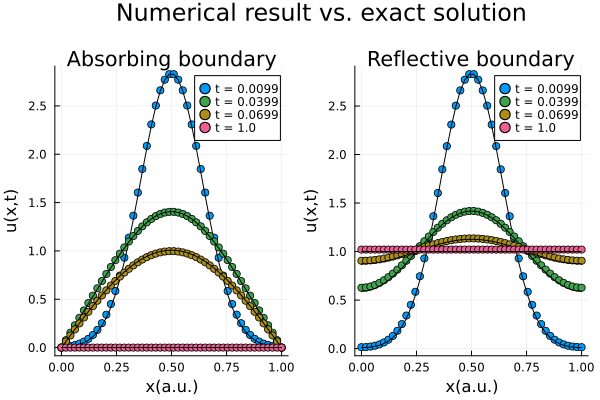
\includegraphics[width=0.9\linewidth]{subplts2.png} % spans the column
\caption{Crank-Nicolson scheme, with $N = 50$, $\Delta t = 10^{-4}$, $D = 1$, CFL number $= 0.25$, plotted against the exact solution for an absorbing and reflective boundary condition respectively, denoted by solid black line.}
\label{fig:subplots2}
\end{figure}

By subtracting the analytical and numerical solutions we can find the an estimate of the maximal numerical error.
\begin{table}[H]
\centering
\begin{tabular}{c|cc}
\hline
Boundary condition & Reflective & Absorbing  \\ \hline
Max error $\epsilon$ & $2.04\times10^{-2}$ & $3.30\times10^{-5}$ \\ 
\end{tabular}
\caption{Maximal error $\epsilon$ given by the difference between exact and numerical solution for a time step of $10^{-4}$, $N = 50$, $D = 1$. CFL number $=0.25$}
\label{error_diffusion}
\end{table}
We notice the error for the von Neumann (reflective) boundary condition is a factor of $10^3$ larger than the Dirichlet (absorbing) boundary condition. The boundary condition causes errors to propagate and reflect back into the domain such that an error at or near the boundary, doesn't dissipate but stays in the system, leading to larger cumulative errors.

\begin{figure}[H]
\centering
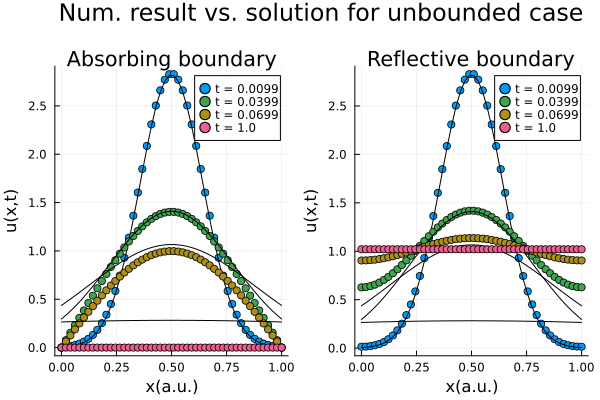
\includegraphics[width=0.8\linewidth]{subplts1.png} % spans the column
\caption{Crank-Nicolson scheme, with $N = 50$, $\Delta t = 10^{-4}$, $D = 1$, CFL number $= 0.25$, plotted against the exact solution for an unbounded case denoted by solid black line.}
\label{fig:subplots1}
\end{figure}
In figure \ref{fig:subplots1} we see that the unbounded solution is a very good approximation for a small time but it gets very bad as $t$ gets larger.
The approximation, gets worse starting from the boundaries. This is to be expected as the two solutions have different boundary conditions, but evolve according to the same PDE.
As we increase the diffusivity constant $D$ the analytical solution for the unbounded case gets even worse.
% \begin{figure}[H]
% \centering
% 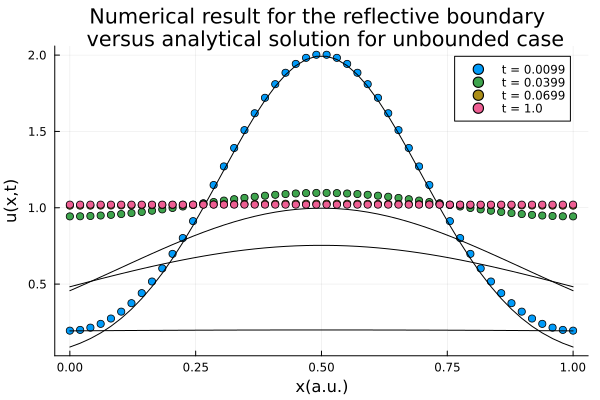
\includegraphics[width=0.7\linewidth]{u_res_reflecting2.png} % spans the column
% \caption{Crank-Nicolson scheme, absorbing boundary, $N = 50$, $\Delta t = 10^{-4}$, $D = 2$, CFL number $= 0.5$, plotted against the analytical solution for the unbounded condition.}
% \label{fig:u_res_reflecting2}
% \end{figure}



\begin{figure}[H]
\centering
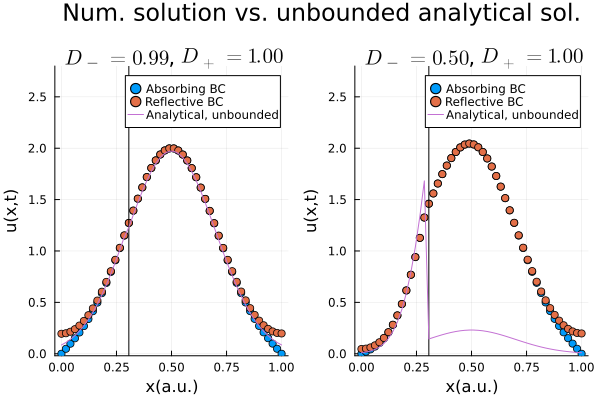
\includegraphics[width=0.8\linewidth]{step_D_subplots.png} % spans the column
\caption{Crank-Nicolson scheme, for both the absorbing and reflective boundary at time $t=0.02$, $N = 50$, $\Delta t = 10^{-4}$. With diffusivity $D_- = 0.99$ and $D_- = 0.50$ as indicated in the figure and $D_+ = 1.00$. In both cases CFL number $\leq 0.25$. The numerical solution is plotted against the analytical solution the unbounded condition. The vertical line denotes the boundary between regions with different diffusivities. The solid violet line represents the analytic solution.}
\label{fig:step_D_subplots}
\end{figure}
Relaxing our initial assumption of $D = const$, allowing for $D$ to be dependent on the position. We notice that the analytical solution for the unbounded
case is a good approximation in the case of similar diffusivity,
as long as we consider small enough time and look away
from the boundaries. It is poor approximation
in the case when we have larger difference between the
diffusivities. This is to be expected considering the discontinuity between the two regions with different $D$. In the special case where $D_- = D_+$, we recover the solution in fig. \ref{fig:subplots2} and \ref{fig:subplots1}.
\begin{figure}[H]
\centering
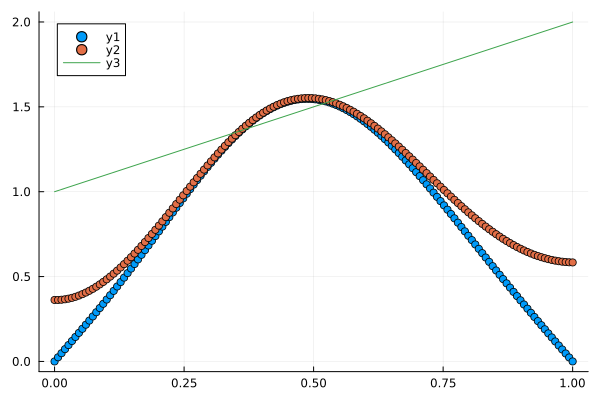
\includegraphics[width=0.7\linewidth]{cont_D.png} % spans the column
\caption{Crank-Nicolson scheme, for both the absorbing and reflective boundary at time $t=0.02$, $N = 50$, $\Delta t = 10^{-4}$, $D \in [0.1,1.1] $, CFL number $\leq 0.275$, plotted against D(x).}
\label{fig:cont_D}
\end{figure}
In the case of space dependent $D(x)$ we expect that the 'density' in higher diffusivity regions to go towards equilibrium faster than regions with lower diffusivity as displayed by figure \ref{fig:cont_D}. Integrating the solution for the reflective b.c. we see that $\int u(x,1) \approx 1 = \Tilde{u}_0$ is conserved, verifying our soulution. 

\section{Wave equation}
\begin{figure}[H]
\centering
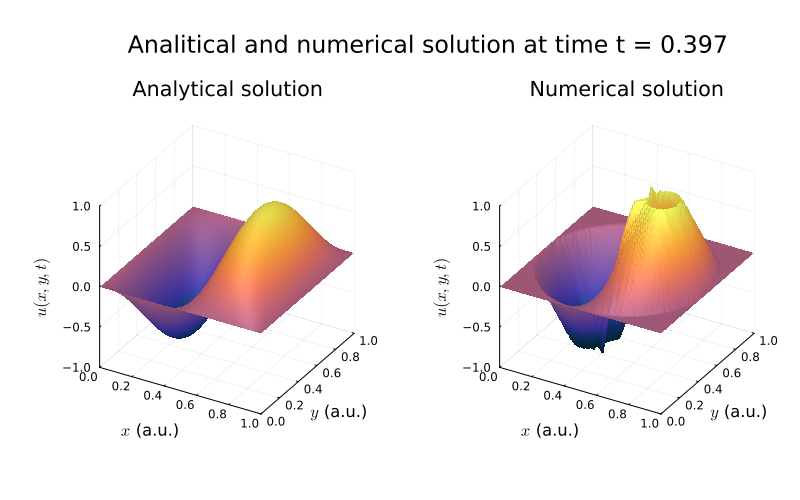
\includegraphics[width=0.7\linewidth]{sine_02.png} % spans the column
\caption{Numerical and analytical solution of the wave equation in 2D with sinusoidal initial condition,  $t=0.397$, $N = 50$, $\Delta t = 10^{-4}$, $c = 1 $, CFL number $ = 0.5 < 1/\sqrt{2}$}.
\label{fig:sine_02}
\end{figure}
Here we see that the CFL condition is fulfilled and the
numerical solution is very similar to the analytical one. The
most immediate consequece of violiting the CFL conditions
is an unphysical result, that is a wave propagating at the
wrong speed. The maximal error $\epsilon = 2.21\times10^{-32}$ given by the difference between exact and numerical solution for a time step $\Delta t =10^{-4}$, $N = 50$, $c = 1$. CFL number $=0.5$ is negligible.Further more we must be careful when subtracting so close numbers due to round-off errors.

\begin{figure}[H]
\centering
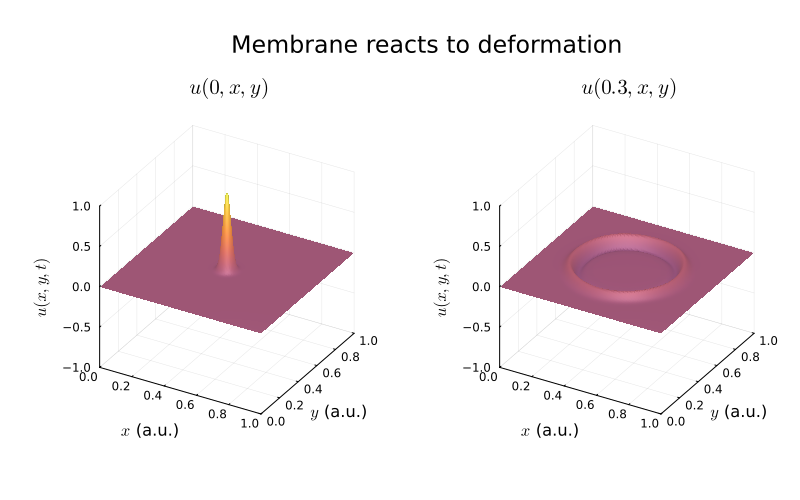
\includegraphics[width=0.7\linewidth]{membrane.png} % spans the column
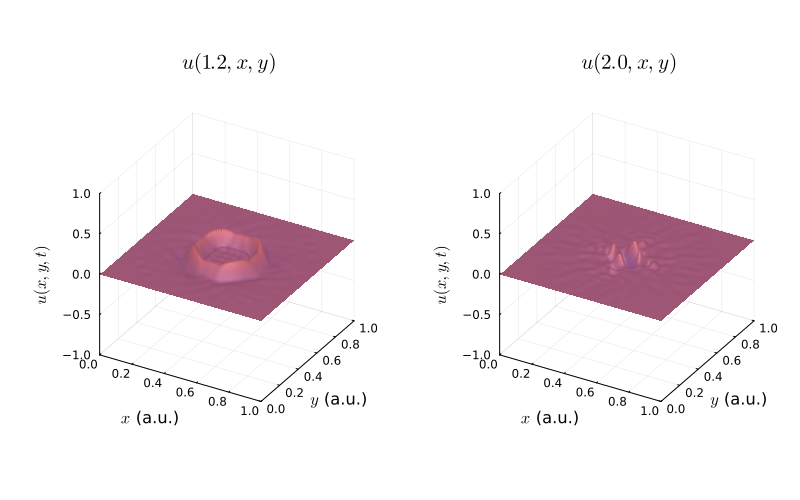
\includegraphics[width=0.7\linewidth]{membrane2.png} % spans the column
\caption{Numerical solution of the wave equation in 2D with initial condition given by eq. \ref{eq:gauss_IC_wave} with $\sigma = 0.001$ and centered at $\mathbf{r_0} = (0.5,0.5)$ for different values of $t$, $N = 100$, $\Delta t = 0.005$, $c = 1$, CFL number $ = 0.5 < 1/\sqrt{2}$.}
\label{fig:membrane}
\end{figure}

Using initial condition (\ref{eq:gauss_IC_wave}), and circular boundary radius $r=0.5$ centered at $\mathbf{r_0}$. This can simulate vibration of a circular membrane, like the eardrum let's say. We observe how waves propagate on such surface.

This model can also simulate the waves on the water after a small initial disturbance (when we trow in a  tiny pebble, for example), assuming we look away from the instant the mass brakes the surface. This model however fails to capture water's particle nature and the fact that we can have splashes. The model also doesn't account for the waves damping due to different factors like viscosity and friction.
\section{Advection equation}
\begin{figure}[H]
\centering
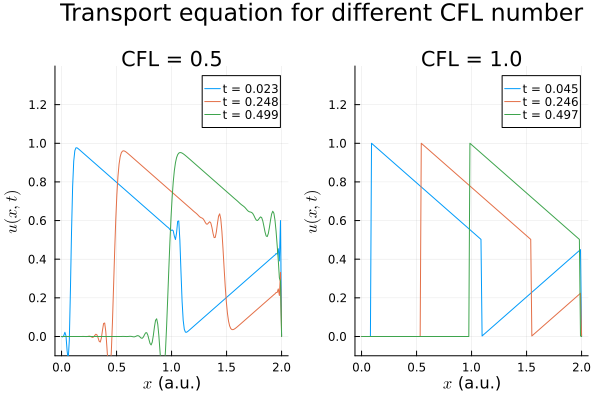
\includegraphics[width=0.9\linewidth]{advection_subplots.png} % spans the column
\caption{Numerical solution of the advection equation (also known as the transport equation) using Lax-Wendroff scheme. The boundary condition is $u(0,t) = u(2,t) = 0$. The initial condition is a step function that is 1 for $x\in[0.3,0.5]$ and zero elsewhere. Subtracting the exact and the numerical solution we obtain that the error in the right graph is $\epsilon = 0.0$, with other words the numerical solution matches the analytical.}
\label{fig:advection_subplots}
\end{figure}
The advection equation models a quantity that is flowing with velocity $c$. As we can see in the figure for CFL number $= 1$, we see no oscillation as the numerical and physical propagation speeds matches. This is akin to shifting the solution by exact grid points without interpolating between points, not introducing additional errors leading to oscillations. When the CFL condition is not fulfilled the solution is unstable leading to nonsensical answer, while for CFL number $< 1$ we see the oscillations around the discontinuities as is typical for the Lax-Wendroff scheme. These oscillations grow with time. 
 
\section{Hopf's equation}
The boundary condition are $u_0 = u_1$ and $u_N = u_{N-1}$, where $u_0$ and $u_N$ are the solutions evaluated at the boundary. Solving Hopf's equation we use a simple Gaussian distribution as an a initial condition:
\begin{align}
    u(0, x) &= \exp{\left(-\frac{(x-x_0)^2}{\sigma}\right)}, & \text{for } (x, y) \in [0,2] 
    \label{Hopf_ic}
\end{align}
with $\sigma = 0.03$ and $x_0 = 0.4$. A shock will develop in finite time if the initial profile $u(x,0)$ has a segment where the derivative with respect to $x$ is negative and sufficiently steep, such that characteristics originating from this segment converge. We see that (\ref{Hopf_ic}) fulfills that condition and naturally we observe shock.

\begin{figure}[H]
\centering
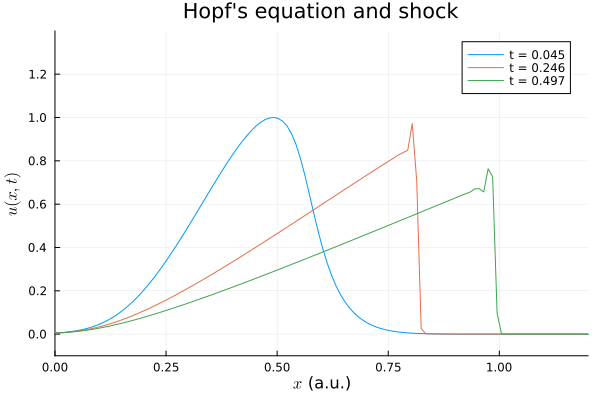
\includegraphics[width=0.9\linewidth]{hopf_CFL1.png} % spans the column
\caption{Numerical solution of Hopf's equation using Lax-Wendroff scheme. $N = 200$, CFL number $= 1$.}
\label{fig:hopf}
\end{figure}
Here we again we used a Lax-Wendroff scheme to solve Hopf's equation and we observe oscillations near the discontinuities. What is more interesting here is that the initially smooth initial condition given by (\ref{Hopf_ic}) evolves in time and develops a discontinuity that propagates to the right and at this point our description of the system as a PDE breaks down. This phenomenon is what we recognize as shock.
\section{Conclusion}
This study has successfully demonstrated the application of numerical methods to solve complex partial differential equations, that are often impossible to solve analytically, offering insights into their behavior under various conditions. They too however have their limitations. We demonstrated some potential issues like oscillations near discontinuities, numerical errors, shock and instabilities. It is important to be familiar with the weaknesses of the methods we use, in order to use them appropriately. Through our analysis, we identified key factors influencing solution accuracy and stability, such as the choice of numerical scheme and the CFL condition. This report highlights the importance of selecting appropriate methods based on the specific problem at hand. Future research should look at more advanced schemes to address these limitations. We need to study a more rigorous way of handling discontinuities and singularities by exploring theories like the theory of distributions.

\makeatletter
\@beginparpenalty=10000 % Vi setter en høy straff for kompilatoren om den setter inn et sideskift mellom streken og starten på referanselisten.
\makeatother

\begin{thebibliography}{99}

\bibitem{assignment} Banon, Jean-Philippe, Simonsen, Ingve. \textit{Computational Physics (TFY4235/FY8904) - Assignment 1
}, NTNU (2024).
\bibitem{presentation1} Dias, R. \textit{Introduction to Assignment 1 - Solving the diffusion equation}, NTNU (2024).
\bibitem{presentation2} Dias, R. \textit{Introduction to Assignment 1 (part II): The
wave equation and the advection equation}, NTNU (2024).
\bibitem{finite_difference} Kværnø, A. \textit{Partial differential equations and finite difference methods}, NTNU (2020).

\bibitem {characteristics} A. Salih. \textit{Method of Characteristics}, (2016). [online] Available at: https://www.iist.ac.in/sites/default/files/people/IN08026/MoC\_0.pdf.
\bibitem{euler_methods} Bui, T. (n.d.). \textit{OpenCommons@UConn Explicit and Implicit Methods In Solving Differential Equations.} [online] Available at: https://digitalcommons.lib.uconn.edu/cgi/viewcontent.cgi?\\article=1118\&context=srhonors\_theses.
\bibitem{von_neumann_ansys} \textit{The Wave Equation. (n.d.)}. Available at: https://www.uni-muenster.de/imperia/md/content/physik\_tp/lectures/ws2016-2017/num\_methods\_i/wave.pdf
\bibitem{}Swan, H., Choi, W., Papanikolaou, S. et al. \textit{“Irregularization” of systems of conservation laws.} Mater Theory 2, 5 (2018). https://doi.org/10.1186/s41313-018-0012-x

\end{thebibliography}

\endgroup

\end{document}